%**************************************************************************************
% License:
% CC BY-NC-SA 4.0 (http://creativecommons.org/licenses/by-nc-sa/4.0/)
%**************************************************************************************

\documentclass[notes]{beamer}

\mode<presentation> {

\usetheme{Madrid}

% Burnt orange
\definecolor{burntorange}{rgb}{0.8, 0.33, 0.0}
\colorlet{beamer@blendedblue}{burntorange}
% Pale yellow
\definecolor{paleyellow}{rgb}{1.0, 1.0, 0.953}
\setbeamercolor{background canvas}{bg=paleyellow}
% Secondary and tertiary palett
\setbeamercolor*{palette secondary}{use=structure,fg=white,bg=burntorange!80!black}
\setbeamercolor*{palette tertiary}{use=structure,fg=white,bg=burntorange!60!black}

% To remove the footer line in all slides uncomment this line
%\setbeamertemplate{footline}
% To replace the footer line in all slides with a simple slide count uncomment this line
%\setbeamertemplate{footline}[page number]

% To remove the navigation symbols from the bottom of all slides uncomment this line
%\setbeamertemplate{navigation symbols}{}
}

\usepackage{amsmath}
\usepackage{bm}
\usepackage{breqn}
\usepackage{fontawesome}
\usepackage{graphicx} % for figures
\usepackage{subcaption} % for subplots 
\usepackage[labelsep=space,tableposition=top]{caption}
\renewcommand{\figurename}{Fig.} 
\usepackage{cleveref}
\usepackage{caption,subcaption}% http://ctan.org/pkg/{caption,subcaption}
\usepackage{booktabs} % Allows the use of \toprule, \midrule and \bottomrule in tables
\usepackage{multirow}
\usepackage{xcolor}
\usepackage{empheq}
\usepackage[most]{tcolorbox}
\usepackage{siunitx}

% To print 2 slides on a page
%\usepackage{handoutWithNotes}
%\pgfpagesuselayout{2 on 1}[border shrink=2mm]
%----------------------------------------------------------------------------------------
%	TITLE PAGE
%----------------------------------------------------------------------------------------
% The short title appears at the bottom of every slide, the full title is only on the title page
\title[CE 311K: Intro to Computer Methods]{CE 311K: Introduction to Computer Methods} 
\author{Krishna Kumar} % name
\institute[UT Austin] % institution 
{
University of Texas at Austin \\
\medskip
\textit{
  \url{krishnak@utexas.edu}} % Your email address
}
\date{\today} % Date, can be changed to a custom date

\begin{document}

\begin{frame}
\titlepage % title page as the first slide
\end{frame}

\begin{frame}
 % Table of contents slide, comment this block out to remove it
 \frametitle{Overview}
 % Throughout your presentation, if you choose to use \section{} and \subsection{} 
 % commands, these %will automatically be printed on this slide as an overview 
 \tableofcontents
\end{frame}

%----------------------------------------------------------------------------------------
% slides
%----------------------------------------------------------------------------------------
%------------------------------------------------
\begin{frame}
	\frametitle{On computable numbers}
	\begin{figure}[ht]
		\centering
		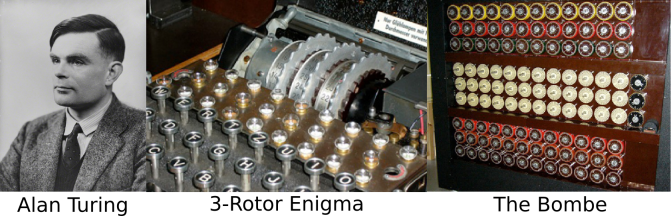
\includegraphics[width=\textwidth]{figs/turing-bombe.png}
		\caption*{Enigma has 150,738,274,937,250 possible states. (credit: Rutherford journal)}
	\end{figure}
\end{frame}

\note{
	Turing began to consider whether a method or process could be devised that could decide whether a given mathematical assertion was provable. Turing analyzed the methodical process, focusing on logical instructions, the action of the mind, and a machine that could be embodied as a physical form. Turing developed the proof that automatic computation cannot solve all mathematical problems. This concept became known as the Turing machine, which has become the foundation of the modern theory of computation and computability.
}

%------------------------------------------------
\begin{frame}
	\frametitle{To infinity and beyond...}
	\begin{figure}[ht]
		\centering
		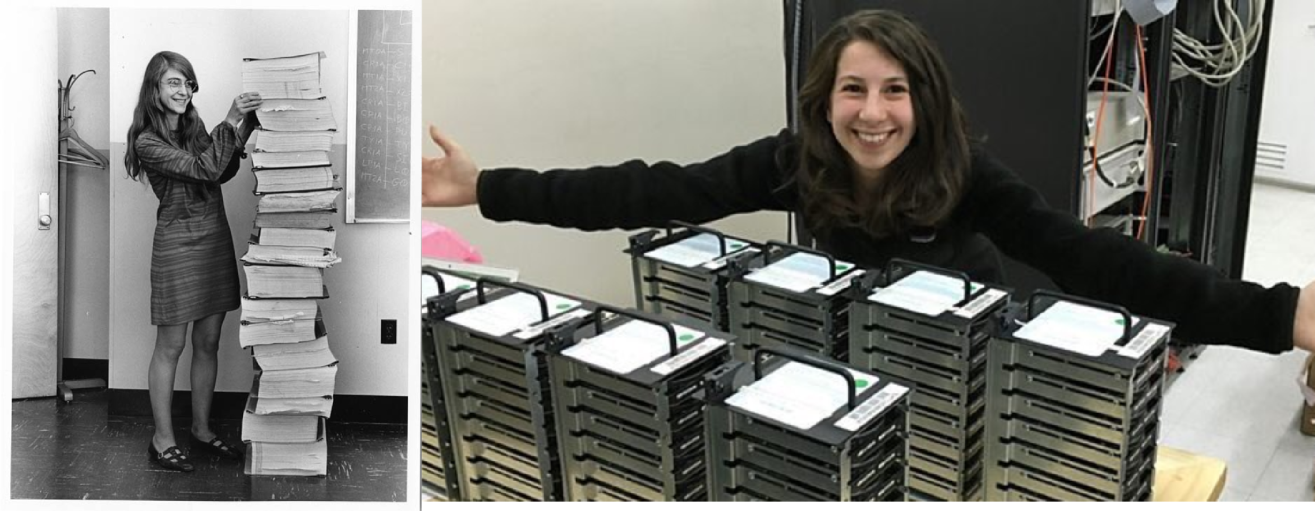
\includegraphics[width=\textwidth]{figs/hamilton-bouman.png}
		\caption*{Margaret Hamilton next to a stack of the Apollo Guidance Computer source code (1969, credit: MIT Museum) and Katie Bouman who developed the algorithm for creating the first-ever image of black hole (2019, credits: PBS).}
	\end{figure}
	\textcolor{blue}{\faQuestionCircleO ~Could you guess the storage size requirements?}
\end{frame}

\note{
	Margaret Hamilton next to a stack of the Apollo Guidance Computer source code (1969, with 11,000 lines of code running on \textbf{72 kilobytes} of computer memory, credits: MIT Museum) and Katie Bouman who developed the algorithm for creating the first-ever image of black hole (2019, credits: PBS) and the HDD of \textbf{5 petabytes} of data. 
	
	If we assume a typical MP3 song as 4MB, we can fit ~56 Apollo guidance code in a song, while the 5 PetaBytes of data can hold 250 million songs (there are roughly ~97 million songs in the world.)
}

%------------------------------------------------
\begin{frame}
	\frametitle{To infinity and beyond...}
	\begin{figure}[ht]
		\centering
		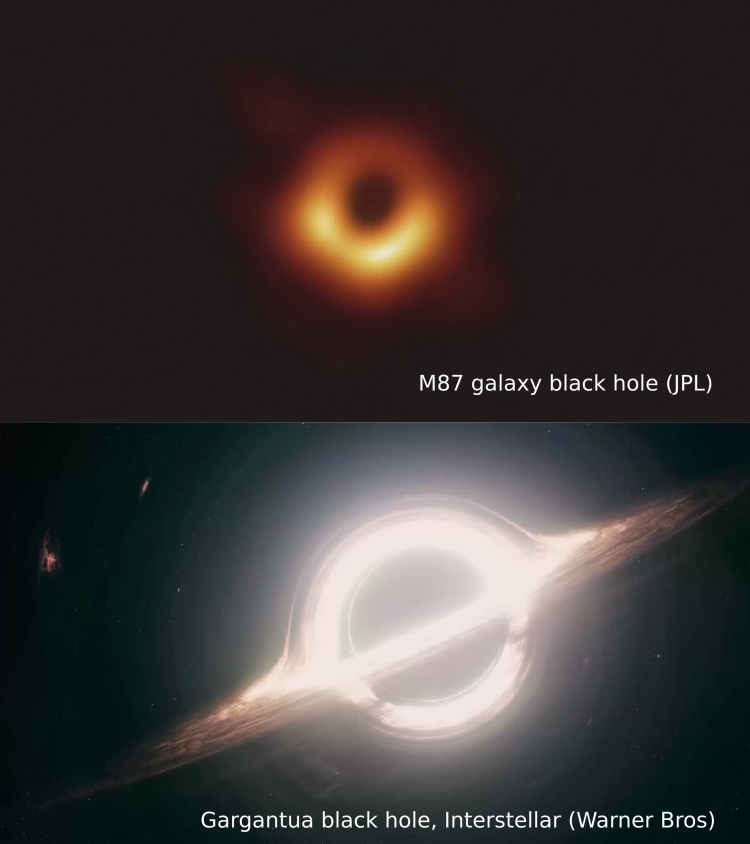
\includegraphics[width=0.55\textwidth]{figs/blackhole.png}
	\end{figure}
\end{frame}

\note{
	Scientists have obtained the first image of a black hole, using Event Horizon Telescope observations of the center of the galaxy M87. The image shows a bright ring formed as light bends in the intense gravity around a black hole that is 6.5 billion times more massive than the Sun. The task of observing this super massive black hole is extremely hard, the size ratio is same as observing an orange on the surface of moon from the Earth.
}

\section{Simulations}
%------------------------------------------------
\begin{frame}
\frametitle{Disney's Frozen: Modeling snow}
\begin{figure}[ht]
	\centering
	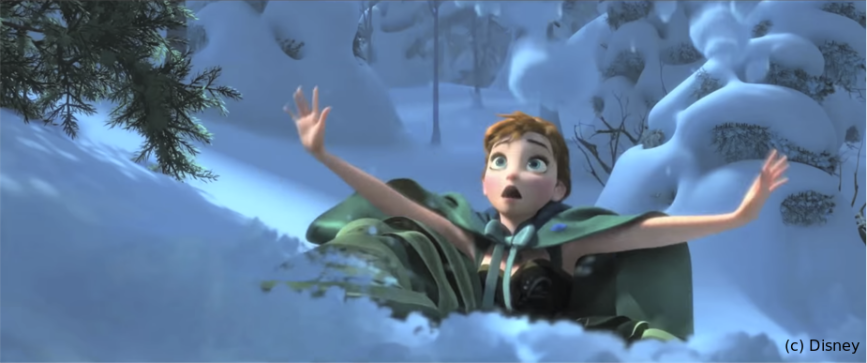
\includegraphics[width=\textwidth]{figs/anna-before-snow.png}
\end{figure}
\end{frame}

%------------------------------------------------
\begin{frame}
\frametitle{How to bury Anna under the snow?}
	\begin{figure}[ht]
		\centering
		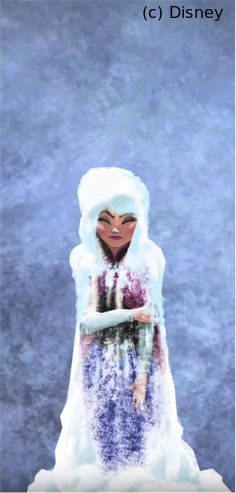
\includegraphics[width=0.3\textwidth]{figs/anna-in-snow.png}
	\end{figure}
\end{frame}

%------------------------------------------------
\begin{frame}
	\frametitle{How to animate like Disney?}
	\begin{figure}[ht]
		\centering
		\includegraphics[width=\textwidth]{figs/anna-snow.png}
		\caption*{\textcolor{blue}{\faCommentsO ~How to achieve the snow simulation?}}
	\end{figure}
\end{frame}

%------------------------------------------------
\begin{frame}
	\frametitle{Modeling the real world: Spherical Cow}
	\begin{figure}[ht]
		\centering
		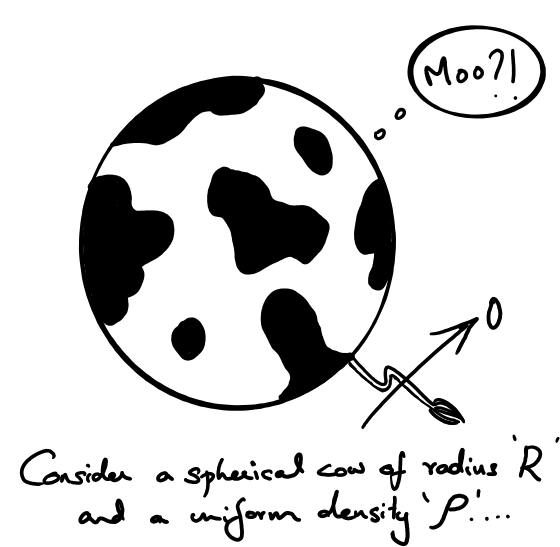
\includegraphics[width=0.65\textwidth]{figs/spherical-cow.png}
	\end{figure}
\end{frame}

%------------------------------------------------
\begin{frame}
	\frametitle{Modeling snow}
	\begin{figure}[ht]
		\centering
		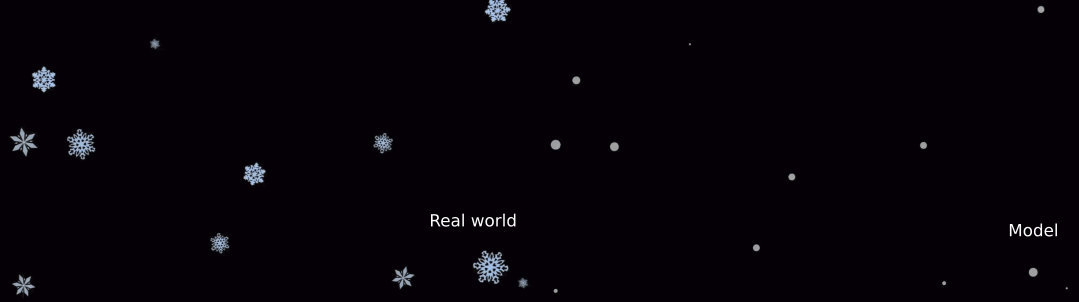
\includegraphics[width=\textwidth]{figs/snow-model.png}
	\end{figure}
\end{frame}

%------------------------------------------------
\begin{frame}
	\frametitle{How to animate like Disney: Effect of snow quantity}
	\begin{figure}[ht]
		\centering
		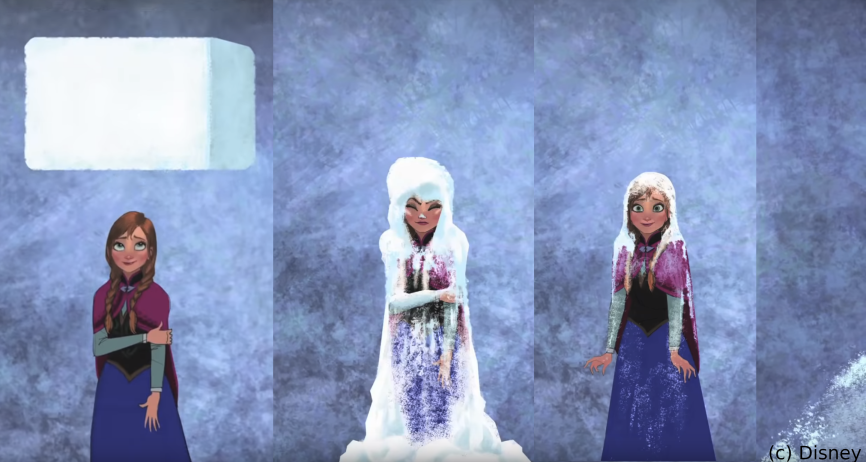
\includegraphics[width=\textwidth]{figs/anna-quantity-snow.png}
	\end{figure}
\end{frame}

%------------------------------------------------
\begin{frame}
	\frametitle{What type of snow?}
	\begin{figure}[ht]
		\centering
		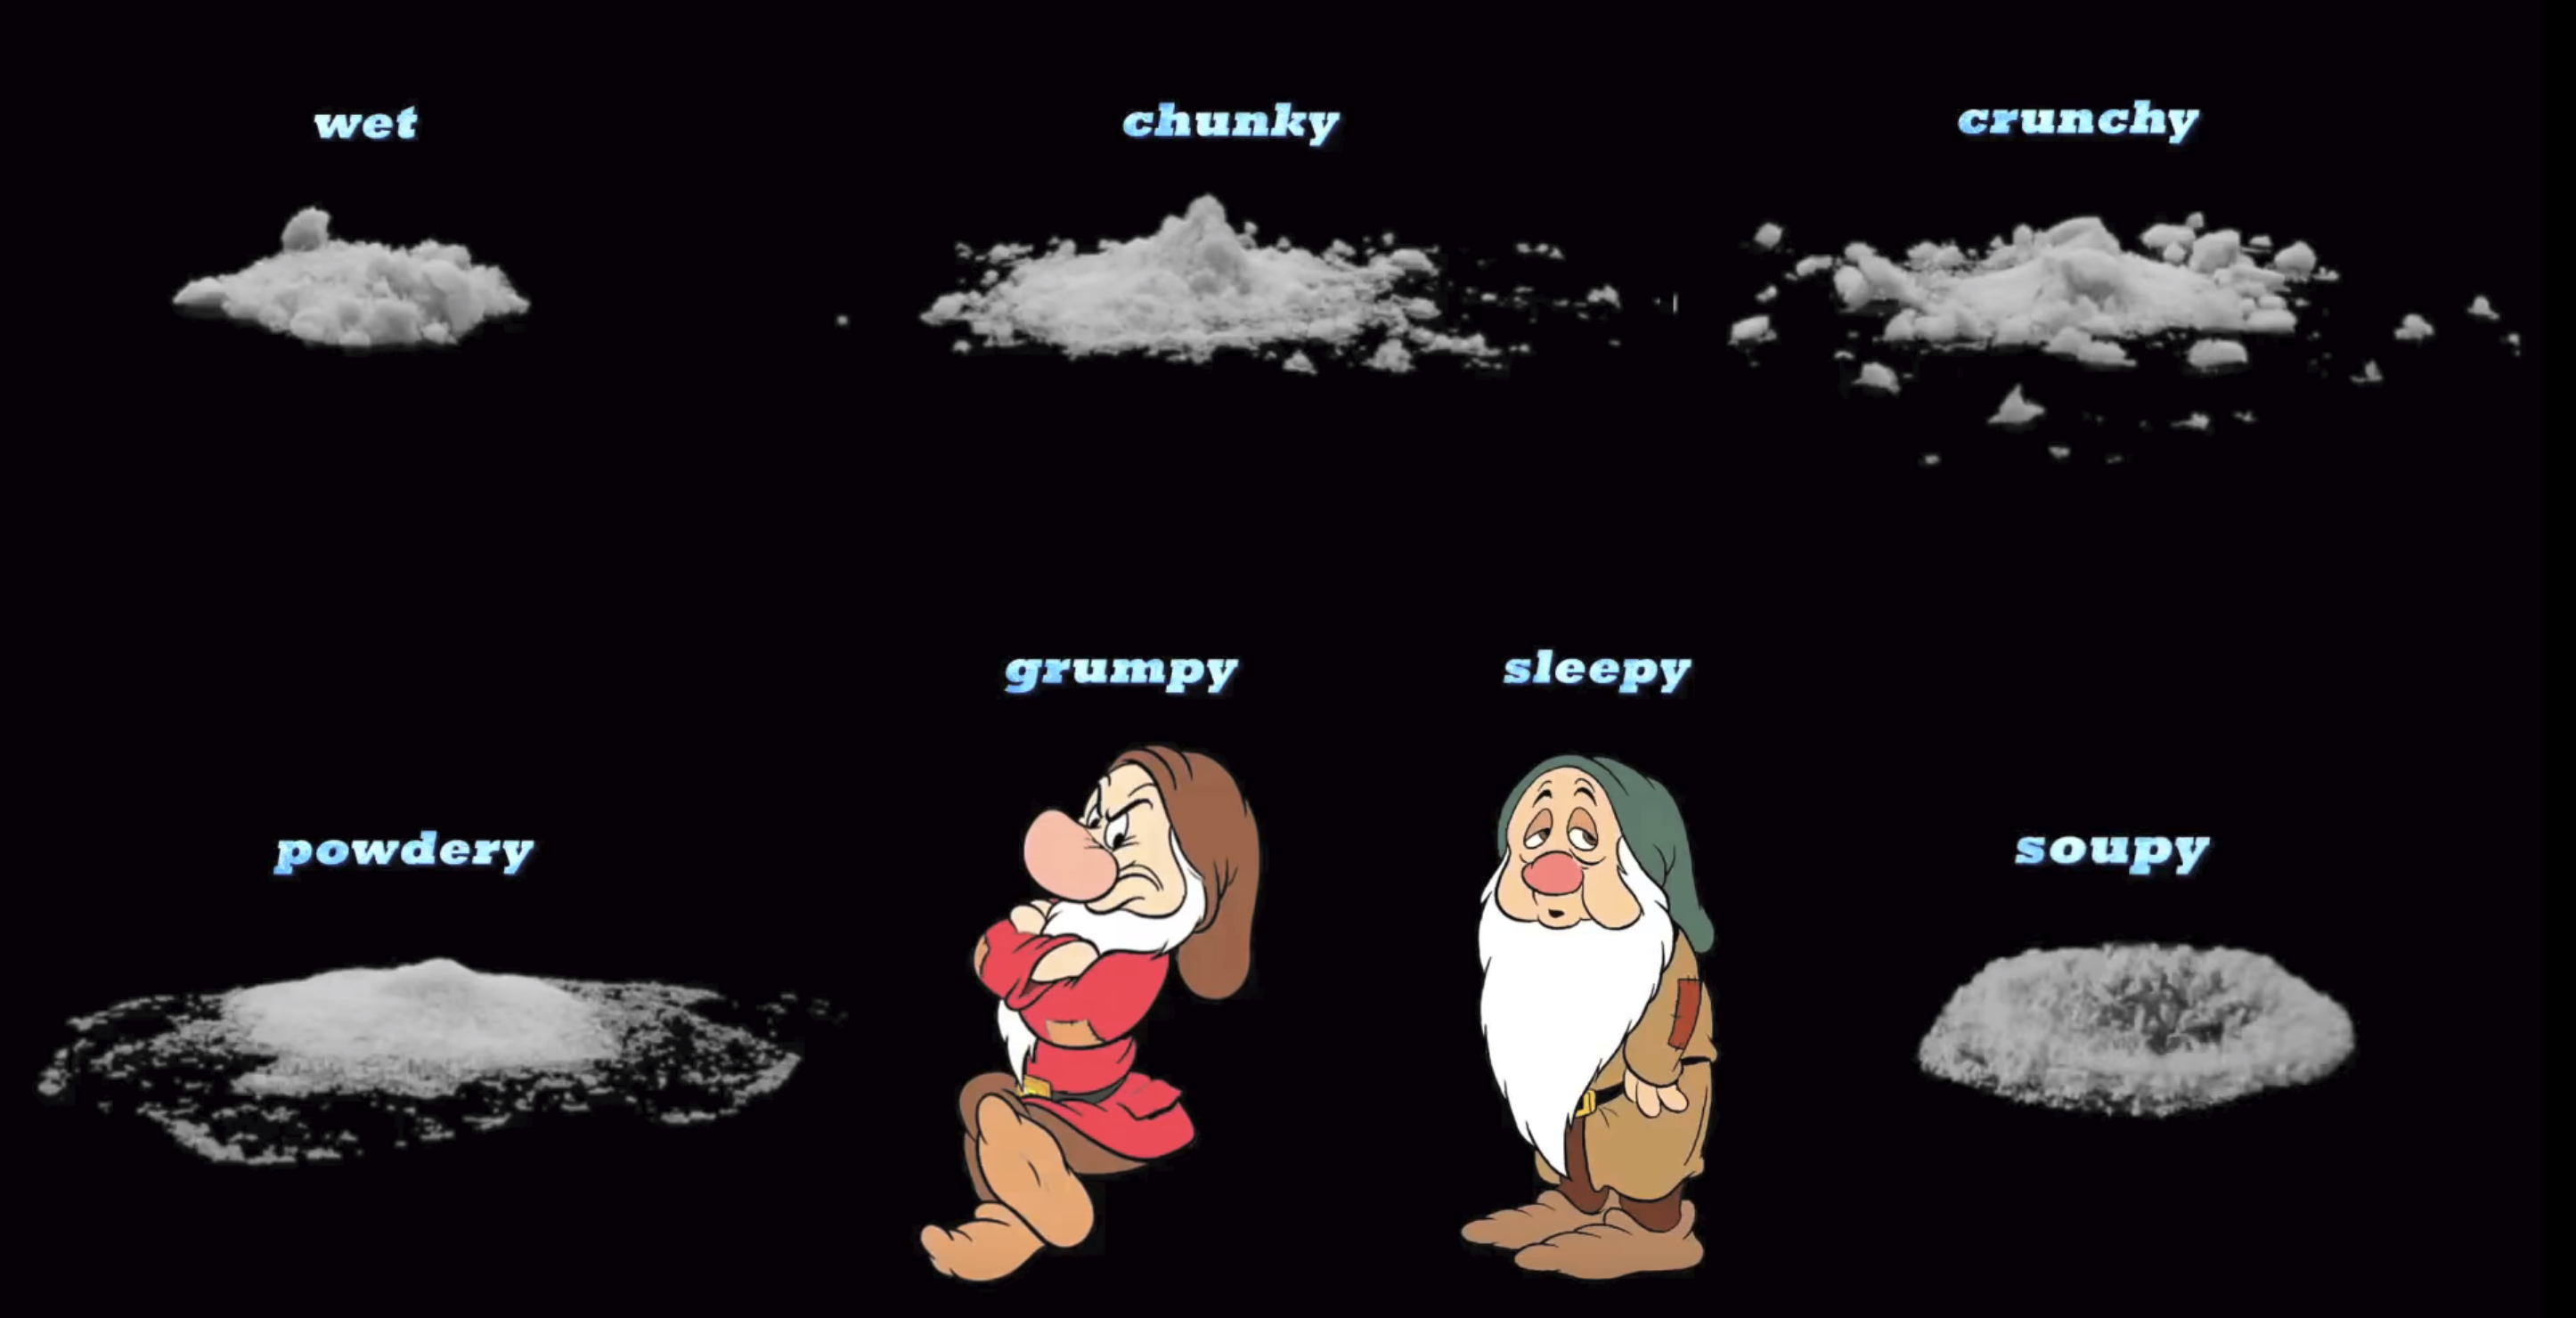
\includegraphics[width=\textwidth]{figs/snow-types.png}
	\end{figure}
\end{frame}

%------------------------------------------------
\begin{frame}
	\frametitle{Snow properties}
	\begin{figure}[ht]
		\centering
		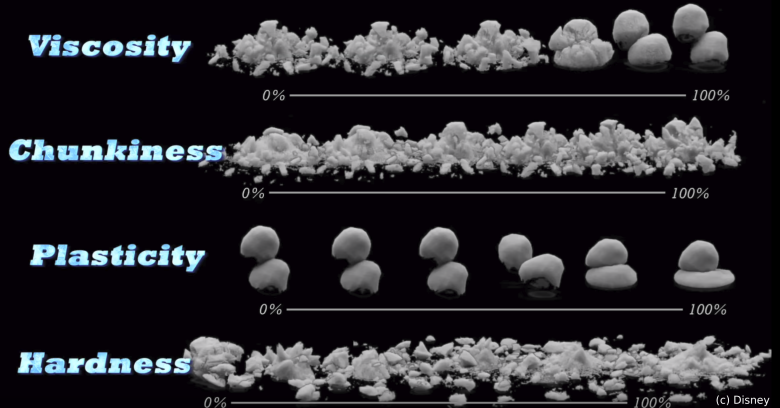
\includegraphics[width=\textwidth]{figs/snow.png}
	\end{figure}
\end{frame}

%------------------------------------------------
\begin{frame}
	\frametitle{Snow material parameters}
	\begin{figure}[ht]
		\centering
		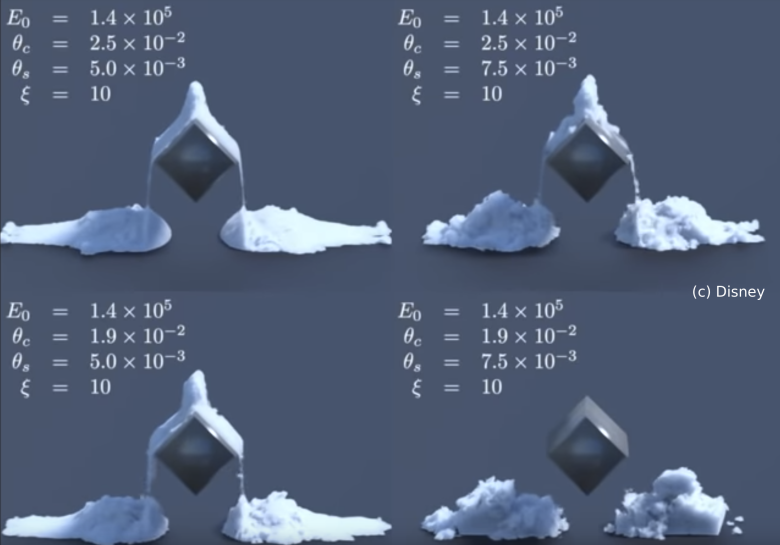
\includegraphics[width=0.9\textwidth]{figs/snow-parameters.png}
	\end{figure}
\end{frame}


%------------------------------------------------
\begin{frame}
	\frametitle{How to model snow?}
	\begin{minipage}[t]{0.59\linewidth}
	\mode<beamer>{
		\begin{itemize}
			\item Representation of snow: Each snow flake is modeled as a particle
			\item Physics: our model or parameters of how the snow behaves
			\item Solver: How the snow would move and interact with the objects in the scene.
			\item Algorithm: A sequence of logical steps required to perform a specific task.
			\item Implementation and verification of our snow model.
		\end{itemize}
		\faLightbulbO~\textcolor{green}{This is a \textbf{simulation}.}
	}
	\mode<handout>{
		\vspace{5cm}
	}
	\end{minipage}%
	\hfill%
	\begin{minipage}[t]{0.39\linewidth}
		\begin{figure}[ht]
			\centering
			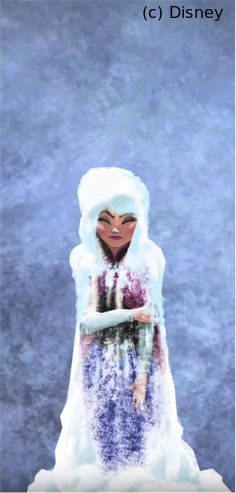
\includegraphics[width=0.7\textwidth]{figs/anna-in-snow.png}
		\end{figure}
	\end{minipage}
\end{frame}

\note{
	 A simulation is an approximate imitation of the operation of a process or system. The first step is to create model, which represents the system's key characteristics, such as its behavior, functions and abstract or physical properties. The model represents the system itself, whereas the simulation represents its operation over time.	
	 
	 There are several numerical techniques that can be used to solve a mathematical problem. They differ in accuracy, length of calulations, and difficulty in programming.
	 
	 Since numerical solutions are an approximation and  the computer program that executes the numerical method might have errors (or bugs), a numerical solution needs to be examined closely.
}

\section{Numerical solution}
%------------------------------------------------
\subsection{Numerical solution of a sliding block}
\begin{frame}
	\frametitle{What is the optimal angle to pull the statue?}
	\begin{figure}[ht]
		\centering
		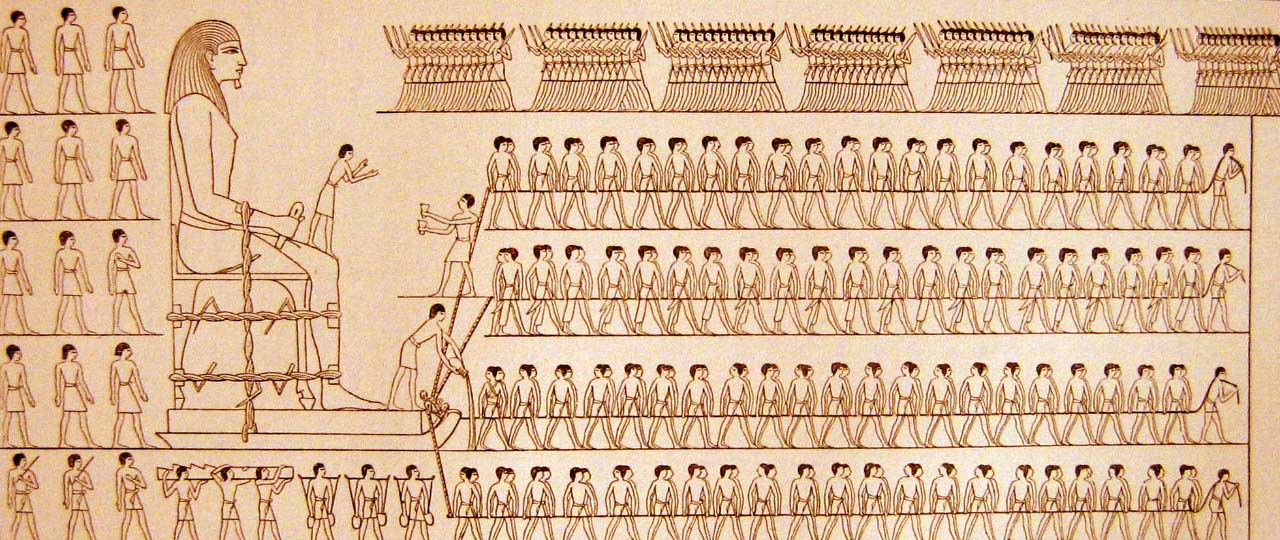
\includegraphics[width=\textwidth]{figs/egypt-pyramid.jpg}
		\caption*{A wall painting from the tomb of Djehutihotep (credit: martinhumanities.com)}
	\end{figure}
\end{frame}

%------------------------------------------------
\begin{frame}
	\frametitle{Numerical solution of a sliding block: Approximation}
	\begin{figure}[ht]
		\centering
		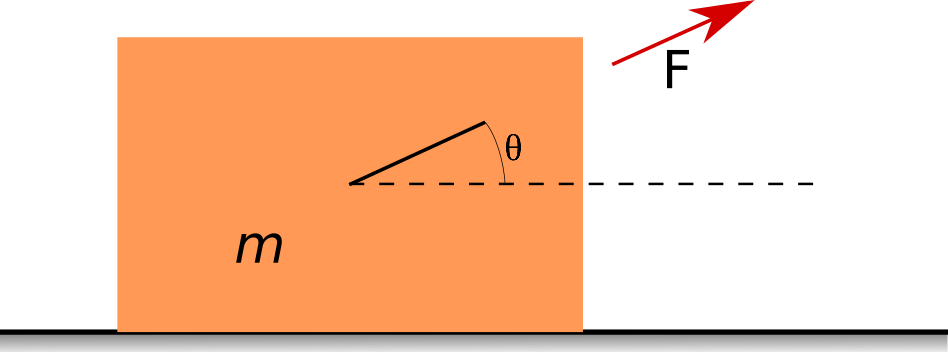
\includegraphics[width=0.85\textwidth]{figs/sliding-block.png}
		\caption*{What is the optimal angle to pull the block applying the least amount of force?}
	\end{figure}
\end{frame}


%------------------------------------------------
\begin{frame}
	\frametitle{Numerical solution of a sliding block: Forces}
	\mode<beamer>{		
		\begin{figure}[ht]
			\centering
			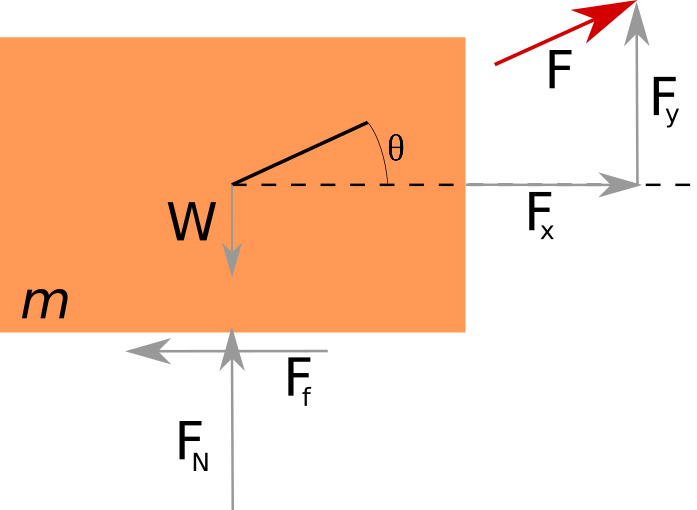
\includegraphics[width=0.85\textwidth]{figs/block-forces.png}
		\end{figure}
	}
	\mode<handout>{
		\begin{figure}[ht]
			\centering
			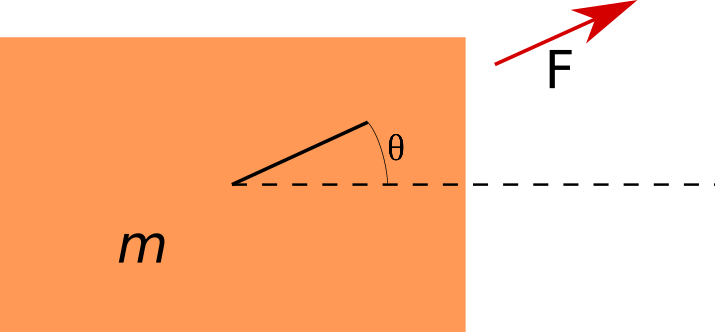
\includegraphics[width=0.85\textwidth]{figs/block-noforces.png}
		\end{figure}
	}
\end{frame}


%------------------------------------------------
\begin{frame}
	\frametitle{Numerical solution of a sliding block: Forces}
	\begin{minipage}[t]{0.7\linewidth}
	\mode<beamer>{		
		\begin{align*}
			& F_x = F \cos \theta \quad \& \quad F_y = F \sin \theta\\
			& F_f = \mu \cdot F_N = \mu \cdot W - \mu F_y = \mu m g - \mu F \sin \theta \\
			& \text{Vertical forces} \sum F_{vert} \uparrow: F_y + F_N - W = 0 \\
			& F_N = \mu m g - F \sin \theta \\
			& \text{Horizontal forces} \sum F_{hor} \rightarrow: F_x + F_f = 0 \\ 
			& F \cos \theta - \mu m g + \mu F \sin \theta = 0 \\
		\end{align*}
	}
	\mode<handout>{
		\vspace{4cm}
	}
	\end{minipage}%
	\hfill%
	\begin{minipage}[t]{0.29\linewidth}
		\begin{figure}[ht]
			\centering
			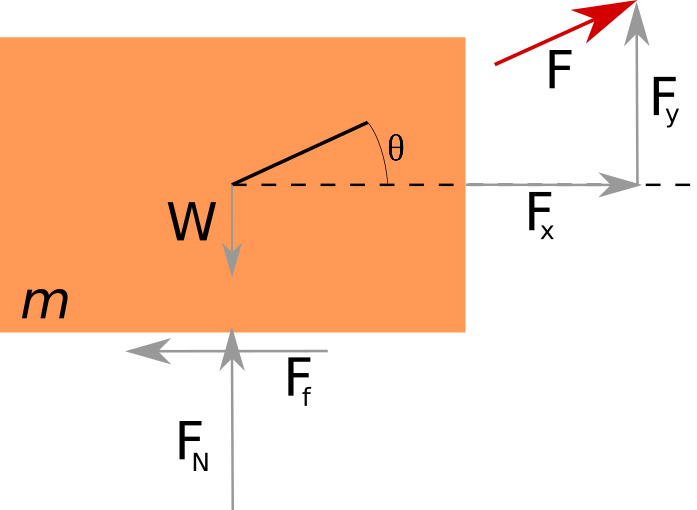
\includegraphics[width=\textwidth]{figs/block-forces.png}
		\end{figure}
	\end{minipage}%
			
	\begin{empheq}[box=\tcbhighmath]{equation*}
		F = \frac{\mu \cdot m g}{(\cos \theta + \mu \sin \theta)}
 	\end{empheq}
\end{frame}

%------------------------------------------------
\begin{frame}
	\frametitle{Numerical solution of a sliding block: Compute force}
	\begin{itemize}
		\item Given $W = 25 kN (\SI{2500}{kg})$, $\theta = 45^o$ and $\mu = 0.75$ ($35^o$):
		\mode<beamer>{	
			\begin{equation*}
				F = \frac{0.75 \times 25 }{\cos(45) + 0.75 \sin(45)} = \SI{15.15}{kN}.
			\end{equation*}
		}
		\mode<handout>{
			\vspace{1cm}
		}
		\item Given $F = 17.5 kN (\SI{2500}{kg})$ and $\mu = 0.75$, what's $\theta$?
		\mode<beamer>{	
			\begin{align*}
			Try~\theta = 60^o:~ & F = \frac{0.75 \times 25 }{\cos(60) + 0.75 \sin(60)} = \SI{16.31}{kN}.\\
			Try~\theta = 70^o:~ & F = \frac{0.75 \times 25 }{\cos(70) + 0.75 \sin(70)} = \SI{17.91}{kN}.\\
			Try~\theta = 65^o:~ & F = \frac{0.75 \times 25 }{\cos(65) + 0.75 \sin(65)} = \SI{17.00}{kN}.\\
			Try~\theta = 67,5^o:~ & F = \frac{0.75 \times 25 }{\cos(67.5) + 0.75 \sin(67.5)} = \SI{17.43}{kN}.
			\end{align*}
			This is \textbf{bisection method!}
		}
		\mode<handout>{
			\vspace{4cm}
		}
	\end{itemize}
\end{frame}


%------------------------------------------------
\begin{frame}
	\frametitle{\faCommentsO ~What are the characteristics of a numerical solution?}
	\mode<beamer>{
		\begin{itemize}
			\item Yields an \textit{approximate} numerical answer (a finite number) for the problem 
			\item These solutions can be very accurate
			\item Most answers are determined in an iterative approach (numerical method: mathematical / computer-aided technique) until a desired minimum/acceptable accuracy is obtained
			\item Typically, a finite set of iterations (steps) are used in the numerical method to obtain a solution
		\end{itemize}
	}
	\mode<handout>{
		\vspace{5cm}
	}
\end{frame}

%------------------------------------------------
\begin{frame}
	\frametitle{Numerical solution of a sliding block: Friction angles}	
	\begin{figure}[ht]
		\centering
		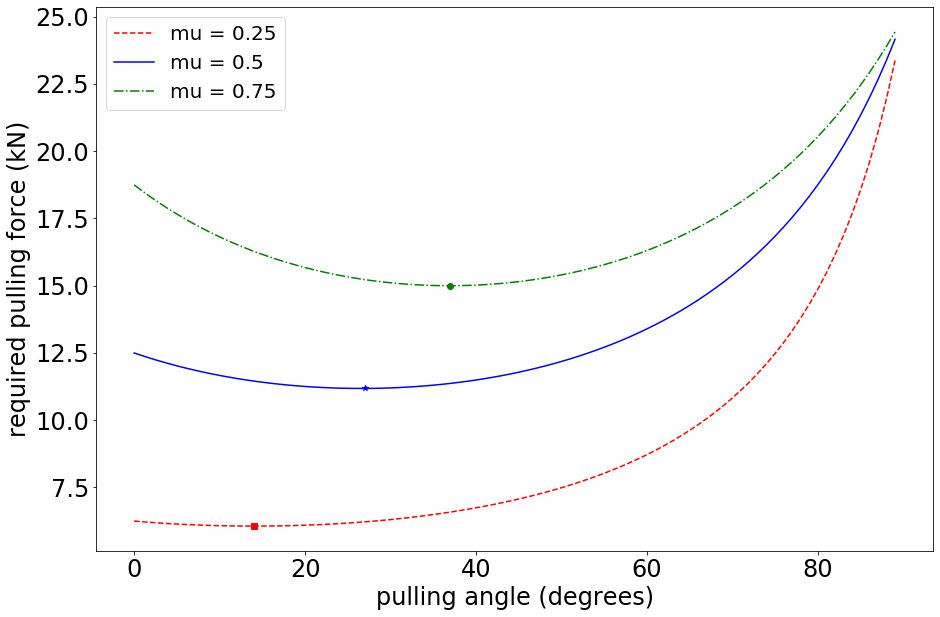
\includegraphics[width=0.85\textwidth]{figs/sliding-block-force-frictions.png}
	\end{figure}
\end{frame}
\end{document}